% YCB1 book: front and back cover. Plain typographic cover in the style of the Game Theory Workbook
% (bold title, rule-dot-rule ornaments, spaced tagline, spaced author name). pdfLaTeX, no Devanagari here.
% Compile: texify -cp --pdf Main_Book_YCB1_covers.tex (make_book_ycb1.bat does it).
\documentclass{article}
\usepackage[paperwidth=6in, paperheight=9in, margin=0.75in]{geometry}
\usepackage[T1]{fontenc}
\usepackage{lmodern}
\usepackage{xcolor}
\usepackage{tikz}
\usepackage{enumitem}
\usepackage[bold]{oswald}
\usepackage[expansion=false]{microtype}
\usepackage{graphicx}
\graphicspath{{images/}{../images/}}

\definecolor{navy}{RGB}{20, 30, 48}
\definecolor{saffron}{RGB}{176, 82, 18}
\definecolor{rulegrey}{RGB}{150, 150, 150}
\definecolor{textgrey}{RGB}{70, 70, 70}

\pagestyle{empty}
\setlength{\parindent}{0pt}

% thin rule, a dot in the middle, thin rule: spans the text width
\newcommand{\ornament}{%
  \begin{tikzpicture}
    \draw[rulegrey,line width=0.4pt] (0,0) -- (0.5*\textwidth-0.2cm,0);
    \fill[saffron] (0.5*\textwidth,0) circle (1.7pt);
    \draw[rulegrey,line width=0.4pt] (0.5*\textwidth+0.2cm,0) -- (\textwidth,0);
  \end{tikzpicture}}

\begin{document}

% ---------------- FRONT COVER ----------------
\thispagestyle{empty}
\begin{center}
\vspace*{0.55in}
{\sffamily\bfseries\color{navy}\fontsize{44}{44}\selectfont YOGA\par}
{\sffamily\bfseries\color{navy}\fontsize{44}{44}\selectfont CERTIFICATION\par}
{\sffamily\bfseries\color{navy}\fontsize{44}{44}\selectfont BOARD\par}
\vspace{0.3em}
{\sffamily\bfseries\color{navy}\fontsize{78}{74}\selectfont LEVEL 1\par}

\vspace{1.0em}
\ornament

\vspace{0.7em}
{\sffamily\bfseries\color{saffron}\fontsize{46}{50}\selectfont\textls[40]{EXAM GUIDE}\par}

\vspace{0.7em}
\ornament

\vspace{1.4em}
{\sffamily\color{textgrey}\fontsize{14}{21}\selectfont\textls[180]{FOR THE YOGA}\par}
{\sffamily\color{textgrey}\fontsize{14}{21}\selectfont\textls[180]{PROTOCOL INSTRUCTOR}\par}

\vspace{1.6em}
{\sffamily\color{saffron}\fontsize{11}{14}\selectfont\textls[100]{COMPLETE TO THE SYLLABUS. NOTHING OUTSIDE IT.}\par}
\end{center}

\vfill
\begin{center}
{\sffamily\bfseries\color{navy}\fontsize{16}{20}\selectfont\textls[220]{YOGESH HARIBHAU KULKARNI}\par}
\vspace{0.7em}
\ornament
\end{center}
\vspace{0.1in}
\clearpage

% ---------------- BACK COVER ----------------
\thispagestyle{empty}
\vspace*{0.05in}
\small

\noindent{\sffamily\bfseries\color{navy}\fontsize{12}{15}\selectfont\textls[100]{ABOUT THE BOOK}}\\[0.3em]
A short, plain guide for the Level 1 exam of the Yoga Certification Board, Yoga Protocol Instructor. It
follows the Board's own syllabus and guideline, covers every topic in them and nothing outside them, and
states the source of its facts.

\vspace{0.8em}
\noindent{\sffamily\bfseries\color{navy}\fontsize{12}{15}\selectfont\textls[100]{WHAT READERS WILL LEARN}}
\begin{itemize}[leftmargin=1.2em,itemsep=0pt,parsep=0pt,topsep=3pt]
  \item the meaning, aim and history of yoga, its principles and schools, and its key texts;
  \item the syllabus practices: cleansing, vyayama, Surya Namaskara, asanas, pranayama, bandha, mudra and meditation;
  \item the basics of the human body, health promotion, daily routine and stress, first aid and CPR;
  \item how to plan a lesson and teach a class;
  \item how the exam works: its parts, the marks and the certificate.
\end{itemize}

\vspace{0.8em}
\noindent{\sffamily\bfseries\color{navy}\fontsize{12}{15}\selectfont\textls[100]{ABOUT THE READER}}\\[0.3em]
Candidates preparing for the Level 1 exam, Yoga Protocol Instructor, and the teachers who train them. No earlier
study of yoga texts or anatomy is assumed.

\vspace{0.8em}
\noindent{\sffamily\bfseries\color{navy}\fontsize{12}{15}\selectfont\textls[100]{ABOUT THE AUTHOR}}\\[0.3em]
Dr Yogesh Haribhau Kulkarni has more than two decades of
experience in Computer-aided Design/Engineering research, software development, and management. He
has Bachelor's, Master's, and Doctoral degrees in Mechanical Engineering, with a specialization in
Geometric Modeling Algorithms. For the past few years, he has been working in fields such as Data
Science, Artificial Intelligence, Machine Learning (ML), Deep Learning (DL), and Natural Language
Processing (NLP). He is also a published author of books on Artificial Intelligence, Mental Models,
and Game Theory.

\vfill

\begin{center}
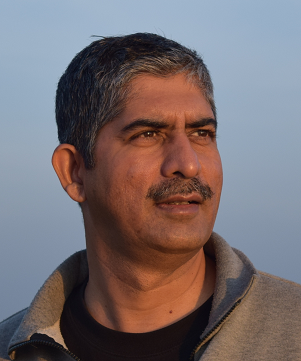
\includegraphics[width=0.11\linewidth,keepaspectratio]{myphoto}

\vspace{0.3em}
{\footnotesize GitHub: github.com/yogeshhk \quad LinkedIn: linkedin.com/in/yogeshkulkarni \quad Medium: yogeshharibhaukulkarni.medium.com}
\end{center}

\begin{center}
{\small \textbf{Publisher:} \ldots \quad \texttt{ISBN:} \ldots}
\end{center}

\end{document}
